% Copyright (c) 2026 William Emerison Six
%
% Permission is granted to copy, distribute and/or modify this document
% under the terms of the GNU Free Documentation License, Version 1.3
% or any later version published by the Free Software Foundation;
% with no Invariant Sections, no Front-Cover Texts, and no Back-Cover Texts.
% A copy of the license is available at https://www.gnu.org/licenses/fdl-1.3.html.
%
% Tower of Hanoi -- fill-in workbook (blank), written at a fifth-grade
% reading level: short sentences, one idea per sentence, numbered steps.
%
% Pages: a cover ("the game", "how to write a move", "the big idea" with
% pictures of each step, "how to swap"), a fully worked example (3 discs built
% from the 2-disc answer), one sheet per n = 1..5, a "for grown-ups" page that
% maps each step to the game's commands, and a cut-out page of paper discs.
%
% Every sheet moves n discs from peg 1 to peg 3, so the copy step is the same
% at every size:
%
%   Step A: top n-1 discs  peg 1 -> peg 2   copy old moves, key 1->1 2->3 3->2
%   Step B: biggest disc   peg 1 -> peg 3   one move
%   Step C: n-1 discs      peg 2 -> peg 3   copy old moves, key 1->2 2->1 3->3
%
% Each copy row has the two halves of the game's rebinding view: the "Copy"
% boxes are the recipe column (the old sheet's move, unchanged) and the "New"
% boxes are the rebound column (the move after the swap key). New moves are
% numbered 1 .. 2^n-1 straight through Steps A, B and C, so the next sheet
% copies "old move 1, 2, 3, ..." by number.
%
% Build:  pdflatex induction-workbook.tex   (needs tikz; no shell-escape).

\documentclass[12pt]{article}
\usepackage[margin=1.4cm]{geometry}
\usepackage[T1]{fontenc}
\usepackage{lmodern}
\renewcommand{\familydefault}{\sfdefault}
\usepackage{tikz}
\usetikzlibrary{calc,arrows.meta,positioning}
\pagestyle{empty}
\setlength{\parindent}{0pt}
\setlength{\parskip}{4pt}

% ---- palette: peg 1/2/3 each keep ONE colour everywhere -------------------
\definecolor{pegc1}{RGB}{31,119,180}    % peg 1 (start)  -- blue
\definecolor{pegc2}{RGB}{230,138,0}     % peg 2 (spare)  -- orange
\definecolor{pegc3}{RGB}{44,160,44}     % peg 3 (goal)   -- green
\definecolor{framegray}{RGB}{120,120,120}
\definecolor{fillgray}{RGB}{245,245,245}
\definecolor{hintgray}{RGB}{110,110,110}
\definecolor{discfill}{RGB}{225,225,225}
\definecolor{pencil}{RGB}{60,60,140}    % the "handwriting" in the example

% A peg number in its peg colour, and "peg N" in its peg colour.
\newcommand{\N}[1]{\textcolor{pegc#1}{\bfseries #1}}
\newcommand{\Peg}[1]{\textcolor{pegc#1}{\bfseries peg~#1}}

\newcommand{\discw}[1]{disc\ifnum#1=1\else s\fi}
\newcommand{\movew}[1]{move\ifnum#1=1\else s\fi}
\newcommand{\arr}{\ensuremath{\rightarrow}}

% ---- the swap key: "1 stays 1", "2 becomes 3", ... -------------------------
\newcommand{\keyitem}[2]{%
  \ifnum#1=#2\relax \N{#1} stays \N{#2}\else \N{#1} becomes \N{#2}\fi}
% #1 #2 #3 = what 1, 2, 3 turn into
\newcommand{\swapkey}[3]{%
  \tikz[baseline=(k.base)]\node[draw=framegray,rounded corners=4pt,
    fill=white,inner sep=5pt,line width=0.8pt](k){\large
    \keyitem{1}{#1}\quad\textbar\quad\keyitem{2}{#2}\quad\textbar\quad
    \keyitem{3}{#3}};}

% ---- pictures of pegs and numbered discs ----------------------------------
% #1 = x position, #2 = peg number
\newcommand{\drawpeg}[2]{%
  \draw[pegc#2,line width=1.3pt] (#1,0) -- (#1,2.0);
  \draw[pegc#2,line width=2.2pt] (#1-1.0,0) -- (#1+1.0,0);
  \node[pegc#2,font=\bfseries\small] at (#1,-0.32) {peg #2};}
% #1 = x position, #2 = bottom disc number, #3 = top disc number (#2 >= #3)
\newcommand{\drawstack}[3]{%
  \foreach \d [count=\i from 0] in {#2,...,#3}{%
    \pgfmathsetmacro{\w}{0.20 + 0.15*\d}%
    \pgfmathsetmacro{\yy}{0.34*\i}%
    \draw[thick,rounded corners=2pt,fill=discfill]
      (#1-\w,\yy+0.02) rectangle (#1+\w,\yy+0.32);
    \node[font=\tiny\bfseries] at (#1,\yy+0.17) {\d};}}
\newcommand{\threepegs}{\drawpeg{0}{1}\drawpeg{2.4}{2}\drawpeg{4.8}{3}}
% The four positions of an n-disc solve. #1 = n (A/B need n >= 2).
\newcommand{\picstart}[1]{\begin{tikzpicture}[scale=0.8]
  \threepegs\drawstack{0}{#1}{1}\end{tikzpicture}}
\newcommand{\picA}[1]{\begin{tikzpicture}[scale=0.8]
  \pgfmathtruncatemacro{\m}{#1-1}%
  \threepegs\drawstack{0}{#1}{#1}\drawstack{2.4}{\m}{1}\end{tikzpicture}}
\newcommand{\picB}[1]{\begin{tikzpicture}[scale=0.8]
  \pgfmathtruncatemacro{\m}{#1-1}%
  \threepegs\drawstack{2.4}{\m}{1}\drawstack{4.8}{#1}{#1}\end{tikzpicture}}
\newcommand{\picgoal}[1]{\begin{tikzpicture}[scale=0.8]
  \threepegs\drawstack{4.8}{#1}{1}\end{tikzpicture}}

% ---- one write-in box, and a "from -> to" pair of them ---------------------
% #1 = text written in it (empty for a blank box)
\newcommand{\wbox}[1]{\tikz[baseline=-0.9ex]{%
  \draw[thick,rounded corners=2pt,fill=white] (0,-0.55) rectangle (1.4,0.55);
  \node[text=pencil,font=\LARGE\bfseries] at (0.7,0) {#1};}}
\newcommand{\wmove}[2]{\wbox{#1}\;{\Large\arr}\;\wbox{#2}}

% ---- one copy row: old move k, its copy, the swap, the new move m ---------
% #1 = y, #2 = k, #3 #4 = copied move, #5 #6 = new move, #7 = m
\newcommand{\gridrow}[7]{%
  \node[anchor=east,font=\small,text=hintgray,align=right] at (1.15,#1)
    {old\\move #2};
  \draw[thick,rounded corners=2pt,fill=white] (1.3,#1-0.58) rectangle (2.9,#1+0.58);
  \node[text=pencil,font=\LARGE\bfseries] at (2.1,#1) {#3};
  \node at (3.3,#1) {\Large\arr};
  \draw[thick,rounded corners=2pt,fill=white] (3.7,#1-0.58) rectangle (5.3,#1+0.58);
  \node[text=pencil,font=\LARGE\bfseries] at (4.5,#1) {#4};
  \draw[-{Stealth[length=3mm]},line width=1.2pt,framegray] (5.7,#1) -- (7.3,#1);
  \node[font=\scriptsize,text=hintgray] at (6.5,#1+0.3) {swap};
  \draw[thick,rounded corners=2pt,fill=white] (7.7,#1-0.58) rectangle (9.3,#1+0.58);
  \node[text=pencil,font=\LARGE\bfseries] at (8.5,#1) {#5};
  \node at (9.7,#1) {\Large\arr};
  \draw[thick,rounded corners=2pt,fill=white] (10.1,#1-0.58) rectangle (11.7,#1+0.58);
  \node[text=pencil,font=\LARGE\bfseries] at (10.9,#1) {#6};
  \node[anchor=west,font=\small\bfseries] at (11.95,#1) {new\\[-2pt]move #7};}
% Column headings over the rows. #1 = old sheet number.
\newcommand{\gridhead}[1]{%
  \node[font=\small\bfseries,align=center] at (3.3,1.2)
    {COPY\\[-1pt]\footnotesize from Sheet #1};
  \node[font=\small\bfseries,align=center] at (9.7,1.2)
    {NEW\\[-1pt]\footnotesize after the swap};}
% Blank grid. #1 = rows, #2 = first new-move number, #3 = old sheet number
\newcommand{\copygrid}[3]{%
  \begin{tikzpicture}[x=1cm,y=1cm,every node/.style={align=left}]
    \gridhead{#3}
    \foreach \k in {1,...,#1}{%
      \pgfmathsetmacro{\y}{-1.42*(\k-1)}%
      \pgfmathtruncatemacro{\m}{#2+\k-1}%
      \gridrow{\y}{\k}{}{}{}{}{\m}}
  \end{tikzpicture}}

% ---- a numbered step heading box ------------------------------------------
% #1 = colour, #2 = title, #3 = body
\newcommand{\stepbox}[3]{%
  \begin{tikzpicture}
    \node[draw=#1,line width=1.2pt,rounded corners=6pt,inner sep=8pt,
          align=left,text width=17.4cm]{%
      {\large\bfseries\textcolor{#1}{#2}}\par\smallskip #3};
  \end{tikzpicture}}

% ======================= one sheet for n = #1 =============================
% #2 = how many moves the old sheet has = 2^(n-1)-1
\newcommand{\hanoipage}[2]{%
  \pgfmathtruncatemacro{\nprev}{#1-1}%
  \pgfmathtruncatemacro{\bignum}{#2+1}%
  \pgfmathtruncatemacro{\cstart}{#2+2}%
  \pgfmathtruncatemacro{\total}{2*#2+1}%
  \pgfmathtruncatemacro{\nnext}{#1+1}%
  \begin{center}
    {\LARGE\bfseries Sheet #1: \ #1 \discw{#1}}\\[4pt]
    \picstart{#1}\quad
    \raisebox{0.7cm}{\Huge\arr}\quad
    \picgoal{#1}
  \end{center}
  \ifnum#1=1
    % ---- the first sheet: one move, nothing to copy ----
    \stepbox{pegc3}{Move disc 1 from peg 1 to peg 3.}{%
      Take disc 1 off \Peg{1}. Put it on \Peg{3}. That is one move.\par
      Write it in the boxes below. Then do it with your disc.\par
      \bigskip
      \centerline{{\large\bfseries new move 1:}\quad\wmove{}{}}
      \bigskip
      You did it! Keep this sheet. You will copy it on Sheet 2.}
  \else
    You need your finished \textbf{Sheet \nprev}. It has \textbf{#2
    \movew{#2}}. You will use it two times.\par
    \medskip
    \stepbox{pegc2}{Step A: \ Move the top \nprev\ \discw{\nprev}
      from peg 1 to peg 2.}{%
      Do these three things on each row:
      \begin{enumerate}\itemsep0pt
        \item \textbf{Copy.} Look at Sheet \nprev. Find \emph{old move 1}.
          Write it in the COPY boxes. Copy it exactly.
        \item \textbf{Swap.} Use the key to change each number.
          Write the new numbers in the NEW boxes.
        \item \textbf{Move.} Do the new move with your discs.
      \end{enumerate}
      Then go to the next row: old move 2, then old move 3, and so on.\par
      \medskip
      \centerline{Key for Step A:\ \ \swapkey{1}{3}{2}}
      \smallskip
      Example: Sheet \nprev\ says \N{1} \arr\ \N{3}.
      The \N{1} stays \N{1}. The \N{3} becomes \N{2}. So you write
      \N{1} \arr\ \N{2}.\par
      Look at one number at a time. Do not change a number twice.}
    \par\medskip
    \begin{center}\copygrid{#2}{1}{\nprev}\end{center}
    \smallskip
    \begin{center}
      \begin{tikzpicture}
        \node[draw=framegray,rounded corners=6pt,inner sep=6pt,fill=fillgray,
              align=center]{%
          \small When Step A is done, your discs look like this:\\
          \picA{#1}};
      \end{tikzpicture}
    \end{center}
    \par\medskip
    \stepbox{pegc1}{Step B: \ Move the biggest disc (disc #1) from peg 1
      to peg 3.}{%
      This is one move. There is nothing to copy. Write it, then do it.\par
      \medskip
      \centerline{{\large\bfseries new move \bignum:}\quad\wmove{}{}}
      \medskip
      \centerline{\small When Step B is done, your discs look like this:}
      \centerline{\picB{#1}}}
    \par\medskip
    \stepbox{pegc3}{Step C: \ Move the \nprev\ \discw{\nprev} from peg 2
      to peg 3.}{%
      Copy Sheet \nprev\ \textbf{again}, from old move 1. Do the same three
      things on each row: \textbf{copy}, \textbf{swap}, \textbf{move}.
      This time the key is different:\par
      \medskip
      \centerline{Key for Step C:\ \ \swapkey{2}{1}{3}}
      \smallskip
      Example: Sheet \nprev\ says \N{1} \arr\ \N{3}.
      The \N{1} becomes \N{2}. The \N{3} stays \N{3}. So you write
      \N{2} \arr\ \N{3}.}
    \par\medskip
    \begin{center}\copygrid{#2}{\cstart}{\nprev}\end{center}
    \par\medskip
    \stepbox{framegray}{Finished! Check your work.}{%
      \begin{itemize}\itemsep0pt
        \item All #1 discs are on \Peg{3}.
        \item You have \textbf{\total\ new moves}, numbered 1 to \total.
        \item Your answer for #1 discs is new moves 1 to \total, in order.
      \end{itemize}
      \ifnum#1<5 Keep this sheet. You will copy it on Sheet \nnext.%
      \else You finished the whole booklet. You can move 5 discs!\fi}
  \fi
  \newpage}

\begin{document}

% ============================ cover page ==================================
\begin{center}
  {\Huge\bfseries Tower of Hanoi}\\[4pt]
  {\Large Grow your tower, one disc at a time}
\end{center}

\section*{What you need}
This booklet. A pencil. Five discs of different sizes. Coins work. You can
also cut out the paper discs on the last page.

\section*{The game}
There are three pegs: \Peg{1}, \Peg{2}, and \Peg{3}. All the discs start
on \Peg{1}. The biggest disc is on the bottom. Disc 1 is the smallest.
\begin{center}\picstart{3}\quad\raisebox{0.7cm}{\Huge\arr}\quad\picgoal{3}\end{center}
Your goal: move all the discs to \Peg{3}. Follow three rules:
\begin{enumerate}\itemsep0pt
  \item Move one disc at a time.
  \item Take only the top disc from a peg.
  \item Never put a bigger disc on a smaller disc.
\end{enumerate}

\section*{How to write a move}
Write the peg you take from, an arrow, and the peg you put on.\par
\N{1} \arr\ \N{3} means: take the top disc off \Peg{1}. Put it on \Peg{3}.

\newpage
\section*{The big idea}
Say you know how to move 3 discs. Then you can move 4 discs.
Here is how. It has three steps:
\begin{center}
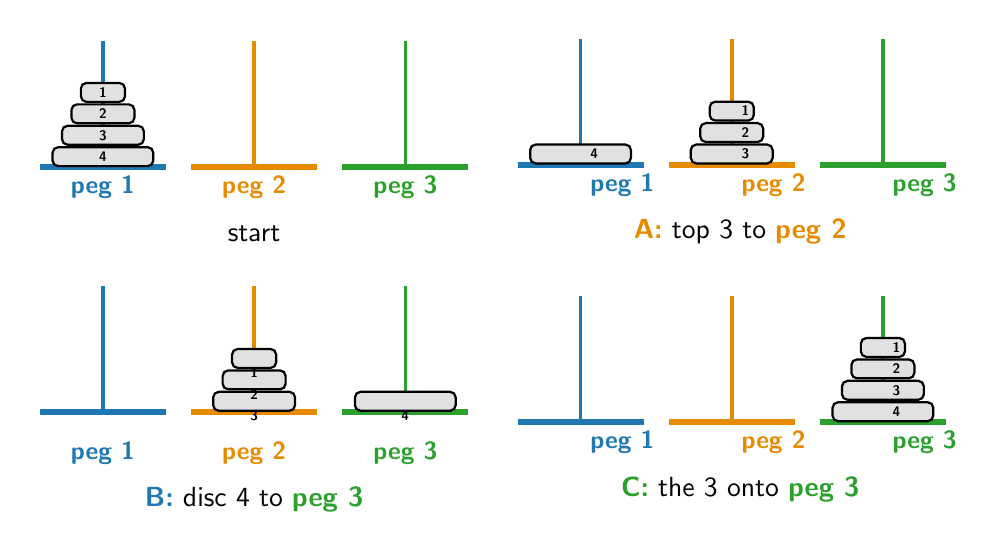
\begin{tikzpicture}
  \node[align=center] (s) {\picstart{4}\\start};
  \node[align=center,right=0.3cm of s] (a)
    {\picA{4}\\\textcolor{pegc2}{\bfseries A:} top 3 to \Peg{2}};
  \node[align=center,below=0.3cm of s] (b)
    {\picB{4}\\\textcolor{pegc1}{\bfseries B:} disc 4 to \Peg{3}};
  \node[align=center,right=0.3cm of b] (c)
    {\picgoal{4}\\\textcolor{pegc3}{\bfseries C:} the 3 onto \Peg{3}};
\end{tikzpicture}
\end{center}
For Steps A and C, you do not need to think. You copy your 3-disc answer
and swap some numbers.

\section*{How to swap}
To swap two numbers means to trade them. Each step has a \textbf{key}. The
key tells you what each number turns into.
\begin{center}
  \begin{tabular}{l@{\qquad}l}
    \textcolor{pegc2}{\bfseries Step A:} & \swapkey{1}{3}{2}\\[14pt]
    \textcolor{pegc3}{\bfseries Step C:} & \swapkey{2}{1}{3}
  \end{tabular}
\end{center}
Change one number at a time. Look at the old number. Find it in the key.
Write what the key says.\par
\textbf{Be careful!} Do not change a number twice. In Step A, a 3 becomes a
2. That new 2 does \emph{not} become a 3 again. Each number changes only once.

\section*{How to use this booklet}
\begin{enumerate}\itemsep0pt
  \item Look at the example on the next page.
  \item Do Sheet 1. It has only one move.
  \item Do Sheet 2. You copy Sheet 1 to make it.
  \item Do Sheet 3. You copy Sheet 2 to make it. Keep going!
\end{enumerate}
Each sheet uses the one before it. Do not skip a sheet.

\newpage
% ============================ worked example ==============================
\begin{center}
  {\LARGE\bfseries Example: making Sheet 3 from Sheet 2}
\end{center}
Here is a finished Sheet 2. It has 3 moves:\par
\centerline{\small old move 1: \N{1}\,\arr\,\N{2} \qquad old move 2:
  \N{1}\,\arr\,\N{3} \qquad old move 3: \N{2}\,\arr\,\N{3}}
\medskip
\textcolor{pegc2}{\bfseries Step A} (key \keyitem{1}{1}, \keyitem{2}{3},
\keyitem{3}{2}). Copy each old move. Then swap.\par
\begin{center}
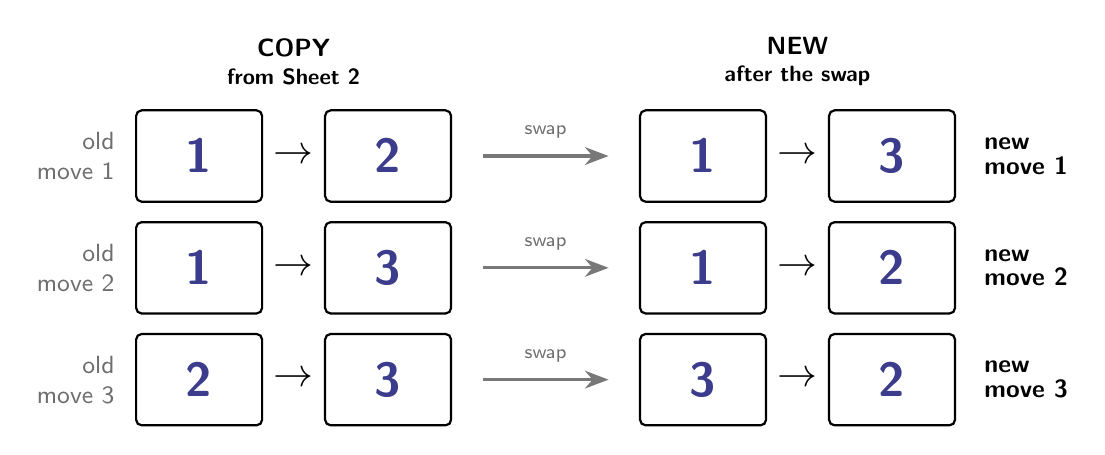
\begin{tikzpicture}[x=1cm,y=1cm,every node/.style={align=left}]
  \gridhead{2}
  \gridrow{0}{1}{1}{2}{1}{3}{1}
  \gridrow{-1.42}{2}{1}{3}{1}{2}{2}
  \gridrow{-2.84}{3}{2}{3}{3}{2}{3}
\end{tikzpicture}
\end{center}
\textcolor{pegc1}{\bfseries Step B.} Move the biggest disc:\quad
{\small new move 4:}\ \wmove{1}{3}\par
\medskip
\textcolor{pegc3}{\bfseries Step C} (key \keyitem{1}{2}, \keyitem{2}{1},
\keyitem{3}{3}). Copy the same old moves again. Then swap.\par
\begin{center}
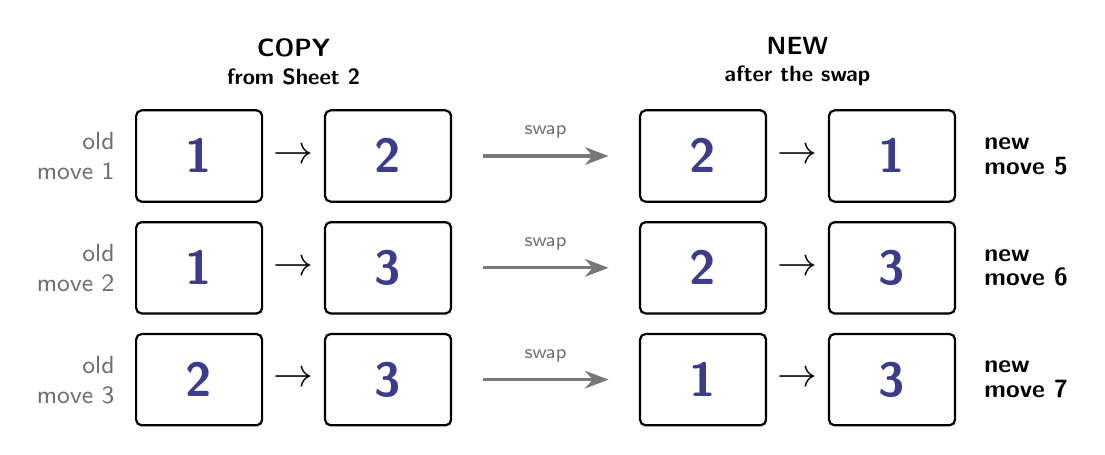
\begin{tikzpicture}[x=1cm,y=1cm,every node/.style={align=left}]
  \gridhead{2}
  \gridrow{0}{1}{1}{2}{2}{1}{5}
  \gridrow{-1.42}{2}{1}{3}{2}{3}{6}
  \gridrow{-2.84}{3}{2}{3}{1}{3}{7}
\end{tikzpicture}
\end{center}
The answer for 3 discs is new moves 1 to 7:\par
\centerline{\N{1}\,\arr\,\N{3},\ \ \N{1}\,\arr\,\N{2},\ \ \N{3}\,\arr\,\N{2},\ \
  \N{1}\,\arr\,\N{3},\ \ \N{2}\,\arr\,\N{1},\ \ \N{2}\,\arr\,\N{3},\ \
  \N{1}\,\arr\,\N{3}}
Try it with 3 discs. It works!
\newpage

% ============================ the sheets ==================================
% #2 = 2^(n-1)-1 moves on the old sheet = rows to copy per step. Large n runs
% onto extra pages on purpose, so every box stays big and lined up.
\hanoipage{1}{0}
\hanoipage{2}{1}
\hanoipage{3}{3}
\hanoipage{4}{7}
\hanoipage{5}{15}

% ============================ for grown-ups ===============================
\section*{For grown-ups}
\textbf{Why it works.} To move $n$ discs from peg 1 to peg 3, first park the
top $n-1$ discs on peg 2, move the biggest disc, then bring the $n-1$ discs
back on top. The smaller stack does not care which pegs it uses, so the
$(n-1)$-disc answer works on any pair of pegs once the peg numbers are
renamed. Every sheet solves the same task (peg 1 to peg 3), so the renaming
is always one of the same two swaps. That renaming is the whole lesson.

\textbf{Checks.} Sheet $n$ has $2^n-1$ moves: 1, 3, 7, 15, 31. Its first move
is \N{1}\,\arr\,\N{3} when $n$ is odd and \N{1}\,\arr\,\N{2} when $n$ is even.
After Step A, discs 1 to $n-1$ sit on peg 2. If a child's move breaks the
rules while they do it with real discs, the mistake is in that row's swap or
copy.

\textbf{The same steps in the computer game.} The hanoi program does exactly
what a sheet does. In the text game (\texttt{hanoi-cli}), after winning 3
discs and saving it as \texttt{solve-3}, start a 4-disc game and type:
\begin{center}
\begin{tabular}{ll}
  \texttt{relabel 1 3 2} & Step A's key (swap 2 and 3)\\
  \texttt{apply solve-3} & Step A: copy and swap all 7 moves\\
  \texttt{relabel 1 2 3} & back to the normal peg numbers\\
  \texttt{1 -> 3}        & Step B\\
  \texttt{relabel 2 1 3} & Step C's key (swap 1 and 2)\\
  \texttt{apply solve-3} & Step C\\
  \texttt{save solve-4}  & keep the answer for Sheet 5
\end{tabular}
\end{center}
When you \texttt{apply} a recipe after a \texttt{relabel}, the game prints a
three-column table. Its \emph{Recipe} column is the COPY boxes, its
\emph{Rebinding} column is the key, and its \emph{Rebound} column is the NEW
boxes. The game's \emph{history} list is the finished sheet.
\newpage

% ============================ cut-out discs ===============================
\begin{center}
  {\LARGE\bfseries Cut-out discs}\\[4pt]
  Cut out the five discs. Lay the page of pegs flat and stack the discs on it.
\end{center}
\vspace{1cm}
\begin{center}
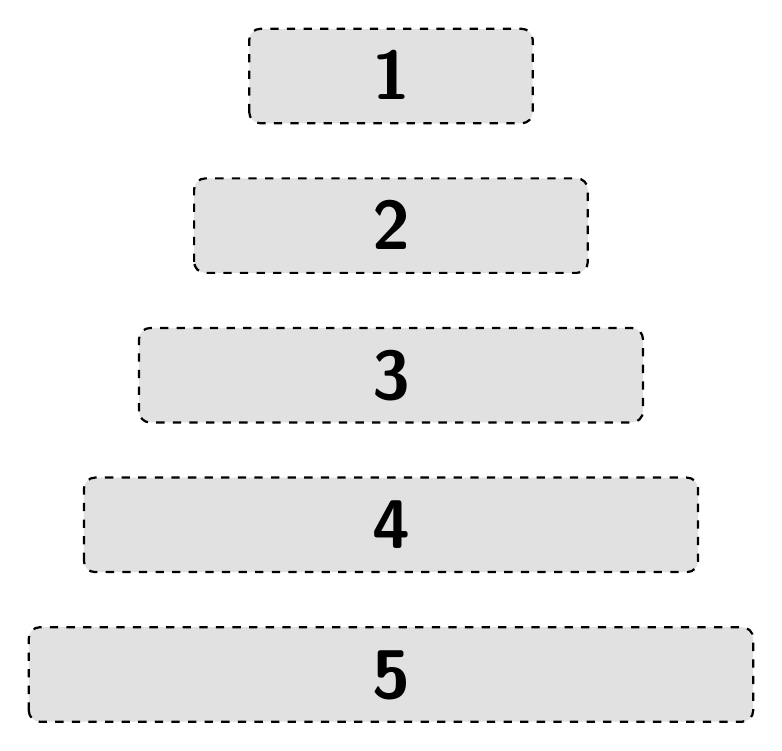
\begin{tikzpicture}
  \foreach \d in {1,...,5}{%
    \pgfmathsetmacro{\w}{1.1 + 0.7*\d}%
    \pgfmathsetmacro{\yy}{-1.9*(\d-1)}%
    \draw[thick,dashed,rounded corners=4pt,fill=discfill]
      (-\w,\yy-0.6) rectangle (\w,\yy+0.6);
    \node[font=\Huge\bfseries] at (0,\yy) {\d};}
\end{tikzpicture}
\end{center}
\vspace{1.5cm}
\begin{center}
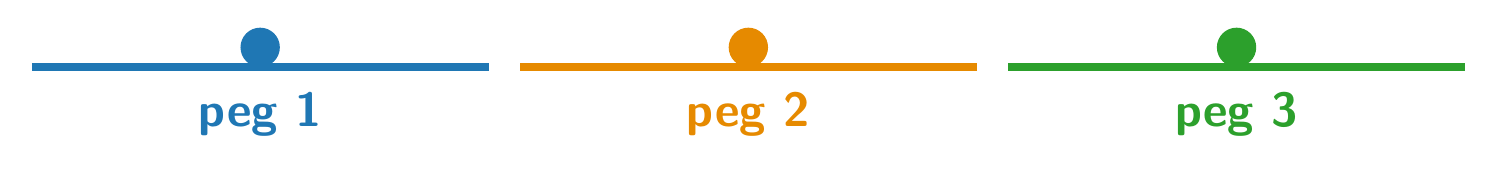
\begin{tikzpicture}
  \foreach \p/\x in {1/0,2/6.2,3/12.4}{%
    \draw[pegc\p,line width=3pt] (\x-2.9,0) -- (\x+2.9,0);
    \fill[pegc\p] (\x,0.25) circle (0.25);
    \node[pegc\p,font=\LARGE\bfseries] at (\x,-0.6) {peg \p};}
\end{tikzpicture}
\end{center}
\end{document}
